\documentclass[runningheads]{llncs}
\usepackage[T1]{fontenc}
\usepackage{graphicx}
\usepackage{amsmath}
\usepackage{booktabs}
\usepackage{tabularx}
\usepackage{multirow}
\usepackage{placeins}
\usepackage{float}
\usepackage[hidelinks]{hyperref}
\setlength{\emergencystretch}{2em}
\begin{document}
\raggedbottom
\title{A Workload Informed Framework for EVM Architecture Modeling and Communication Cost Evaluation in Floorplanning}
\titlerunning{Workload Informed EVM Modeling and Floorplanning}
% Working title and author metadata, affiliation to be supplied before submission.
\author{Dongfang WU \and Shuo Ren \and Tony Tsz Chun MAN \and Priscilla FERNANDEZ LOAIZA \and Yolanda Wong Ying YIP \and Clement CY THAM \and Calvin CP PANG \and M{\aa}rten E BREL{\'E}N}
\authorrunning{D. Wu et al.}
\institute{\email{dongfang.wu@link.cuhk.edu.hk}}
\maketitle
\begin{abstract}
State access, updates, and commitment computation motivate the exploration of hardware acceleration for the Ethereum Virtual Machine (EVM). This study develops a workload characterization and architecture evaluation framework for Ethereum Mainnet, OP Mainnet, and Arbitrum One. A stratified probability sampling approach selects 72 dates across twelve three month phases, providing consistent observation windows for comparing transaction workloads. Building on the collected block and transaction data, we develop an abstract eight module architecture and introduce a workload informed connectivity model using transaction counts, contract creation activity, and block data size as proxy indicators. We evaluate optimized planar and two layer layouts under consistent architectural assumptions. At a vertical interconnection cost ratio of one, the two layer model reduces mean communication costs by 5.59\%, 4.82\%, and 5.25\% across the three networks, respectively. These results demonstrate conditional advantages of three dimensional layouts within the proposed model, while execution tracing and hardware validation remain necessary to establish practical performance benefits.

\keywords{Ethereum Virtual Machine \and Workload characterization \and State processing \and Hardware acceleration \and Three dimensional integration}
\end{abstract}

\section{Introduction}
Conceived by Vitalik Buterin as a decentralized world computer, Ethereum introduced the EVM for programmable smart contracts. During the initial coin offering (ICO) boom, projects issued ERC-20 tokens, raised Ether (ETH), and distributed tokens to investors. Early upgrades addressed execution efficiency and gas costs. EIP-145 added native bitwise shifts~\cite{eip145}, and EIP-1052 added \texttt{EXTCODEHASH} for retrieving code hashes directly~\cite{eip1052}. Both entered the Constantinople upgrade~\cite{constantinople}.

Smart contract applications expanded to decentralized finance (DeFi), including Uniswap, blockchain games such as Axie Infinity, and virtual worlds such as The Sandbox. Growing activity increased pressure on mainnet capacity, with congestion and high fees affecting usability during peak demand in 2021.

Layer 2 (L2) rollups execute transactions outside Ethereum's Layer 1 (L1), batch results, and publish protocol data to Ethereum for settlement and data availability~\cite{rollups}. Sequencers order transactions and provide preliminary confirmations. Fraud or validity proofs check execution according to the rollup design~\cite{rollups,zkrollups}. Sequencing capacity, execution efficiency, and state management remain scaling constraints.

Dedicated hardware has shown potential for acceleration. EVMx reported faster execution of commonly used opcodes on an FPGA engine than in CPU environments~\cite{evmx}. Performance also depends on module organization and data exchange. Three dimensional integration offers alternative placements and communication paths, with benefits governed by workloads and vertical interconnection costs~\cite{xu2013,hsu2013}.

We characterize L1 and L2 workloads, model communication in an abstract EVM architecture, and compare planar and three dimensional layout costs through three research questions:
\subsubsection{RQ1. Workload Characterization}
How do observable transaction workloads vary across L1 and L2 networks under different sampled load conditions?
\subsubsection{RQ2. Communication Modeling}
How can observable blockchain workload indicators be incorporated into an abstract intermodule connectivity model for architectural evaluation?
\subsubsection{RQ3. Physical Layout Evaluation}
Under what conditions can two layer integration reduce modeled communication costs compared with optimized planar layouts using workload based connectivity models?

\section{Dataset and Sampling Design}
Ethereum Mainnet provides the L1 reference, while OP Mainnet and Arbitrum One represent EVM compatible L2 environments based on the OP Stack and Arbitrum Nitro. Sampling supports comparison across these architectures while balancing temporal coverage and processing requirements.

\subsection{Observation Window and Probability Sampling}
The observation window spans 1,096 days from November 16, 2023, at 00:00 UTC inclusive to November 16, 2026, at 00:00 UTC exclusive. Stratified probability sampling captures variation in markets, application demand, and network development within feasible storage and processing requirements.

The window comprises twelve consecutive three month phases, each stratified into weekdays and weekends. With seed 20231116, four weekdays and two weekend days are drawn without replacement per phase, yielding 72 dates shared across networks. Each date includes all blocks from 12:00 UTC inclusive to 13:00 UTC exclusive. Matched dates and a fixed hour provide consistent calendar conditions for cross network comparisons.

\subsection{Event Supplements and Analysis Populations}
March 12 and March 14, 2024, surrounding Ethereum's Dencun upgrade, form a separately labeled event sample. All networks cover the 74 retained dates, yielding 222 chain hours: 216 probability sample hours and six event hours. The panel is balanced by chain hour, with varying block counts. Population estimation uses the probability sample of 72 hours per network, as shown in Table~\ref{tab:sample}.

\begin{table}[H]
\caption{Probability sample coverage. Failed denotes the total failed transaction count. Failure share is the pooled failed count divided by all transactions.}\label{tab:sample}
\centering\footnotesize
\setlength{\tabcolsep}{2pt}
\begin{tabular*}{\textwidth}{@{\extracolsep{\fill}}lrrrrr@{}}
\toprule Network & Hours & Blocks & Transactions & Failed & \shortstack{Failure\\share (\%)} \\\midrule
Ethereum & 72 & 21,460 & 4,816,644 & 68,861 & 1.43 \\
OP Mainnet & 72 & 129,600 & 3,664,812 & 190,514 & 5.20 \\
Arbitrum One & 72 & 1,029,423 & 7,202,553 & 725,471 & 10.07 \\
\bottomrule
\end{tabular*}
\end{table}
\FloatBarrier

Unweighted tables summarize the sample. Estimating the three year mean at the fixed observation hour uses stratum weights:
\begin{equation}
\widehat{\mu}=\frac{1}{1096}\sum_h\frac{N_h}{n_h}\sum_{d\in s_h}y_d\label{eq:stratified}
\end{equation}
Here $y_d$ is the hourly outcome on date $d$, $N_h$ and $n_h$ are population and sample date counts in stratum $h$, and $s_h$ is its sampled date set. The same weights apply to matched cross chain differences. Inference concerns daily activity from 12:00 to 13:00 UTC over the observation window.

\subsection{Data Fields and Missingness}
SQD Portal supplies block headers and receipt data. Identifiers, timestamps, hashes, state roots, and source metadata support verification and replay selection. Analysis uses 15 numerical fields: gas usage, gas limits, gas utilization, base fees, block sizes, transaction counts, total transaction gas consumption, failed transactions, contract creations, transactions with destinations, and counts for types 0, 1, 2, 3, and other.

The common analysis uses fields available across networks and protocol versions. Blob gas coverage varies, and eight reserved execution metrics, including storage operations, trie accesses, Keccak operations, dependency depth, and RTL communication bytes, remain unavailable. Observable workload indicators therefore supply proxy communication weights for an abstract eight module architecture and its two dimensional and three dimensional layouts.

\section{Descriptive Workload Statistics}
We compare block production, transaction volumes, and failed transactions across the three networks using the probability sample in Section~2. Table~\ref{tab:hourly} summarizes the hourly statistics.

% Selected source tables are inserted below.

OP Mainnet records 1,800 blocks in each of the 72 sampled hours, giving zero SD and IQR. This agrees with its specified two second block interval~\cite{opinterval}.

\begin{table}[H]
\caption{Hourly statistics recomputed from 72 probability dates per network. SD is the sample standard deviation. IQR is the 75th minus the 25th percentile, using linear interpolation. All entries are counts per hour.}\label{tab:hourly}
\centering\footnotesize
\setlength{\tabcolsep}{2pt}
\begin{tabular*}{\textwidth}{@{\extracolsep{\fill}}llrrrr@{}}
\toprule Network & Metric & Mean & SD & Median & IQR \\\midrule
\multirow{3}{*}{Ethereum} & Blocks & 298.06 & 1.56 & 298.00 & 2.00 \\
 & Tx & 66,897.83 & 22,820.19 & 59,843.00 & 27,971.75 \\
 & Failed tx & 956.40 & 423.45 & 790.50 & 449.00 \\
\addlinespace
\multirow{3}{*}{OP Mainnet} & Blocks & 1,800.00 & 0 & 1,800.00 & 0 \\
 & Tx & 50,900.17 & 27,892.30 & 47,029.50 & 35,357.25 \\
 & Failed tx & 2,646.03 & 2,729.76 & 1,756.50 & 2,447.25 \\
\addlinespace
\multirow{3}{*}{Arbitrum One} & Blocks & 14,297.54 & 258.87 & 14,371.50 & 81.00 \\
 & Tx & 100,035.46 & 41,788.60 & 93,294.50 & 51,736.50 \\
 & Failed tx & 10,075.99 & 9,719.30 & 7,368.50 & 8,820.50 \\
\addlinespace
\bottomrule
\end{tabular*}
\end{table}
\FloatBarrier

\subsection{Within Phase Load Groups}
Within each chain and phase, the six sampled hours are ranked by total gas used, breaking ties by earlier date. Consecutive pairs form low (L1), medium (L2), and high (L3) groups, giving 24 hours per group per chain. These groups express ranks within the sample.

Transaction and block aggregates describe activity, and Pearson correlations summarize within chain covariation. Attribution to state access, commitment computation, and memory stalls requires execution evidence. Correlations involving constant variables are undefined.

\subsection{Temporal Variation and Multivariate Workload Profiles}
Figure~\ref{fig:workload_combined} uses the 72 probability dates per network, recomputed from compressed block records and the common calendar. Hourly failure fractions divide failed transactions by all transactions.

The top row compares equally weighted hours. Median transaction counts are 59,843, 47,029.5, and 93,294.5 for Ethereum, OP Mainnet, and Arbitrum One, with median failure fractions of 1.35\%, 3.93\%, and 7.36\%. The curves retain upper tails. Table~\ref{tab:sample} reports transaction weighted pooled failure shares.

The bottom row relates transaction volume to failure fraction, colored by within phase gas rank. Overlapping groups show variation in transaction mix and failures within each rank. These associations support workload selection, with causal interpretation requiring further evidence.

\begin{figure}[H]
\centering
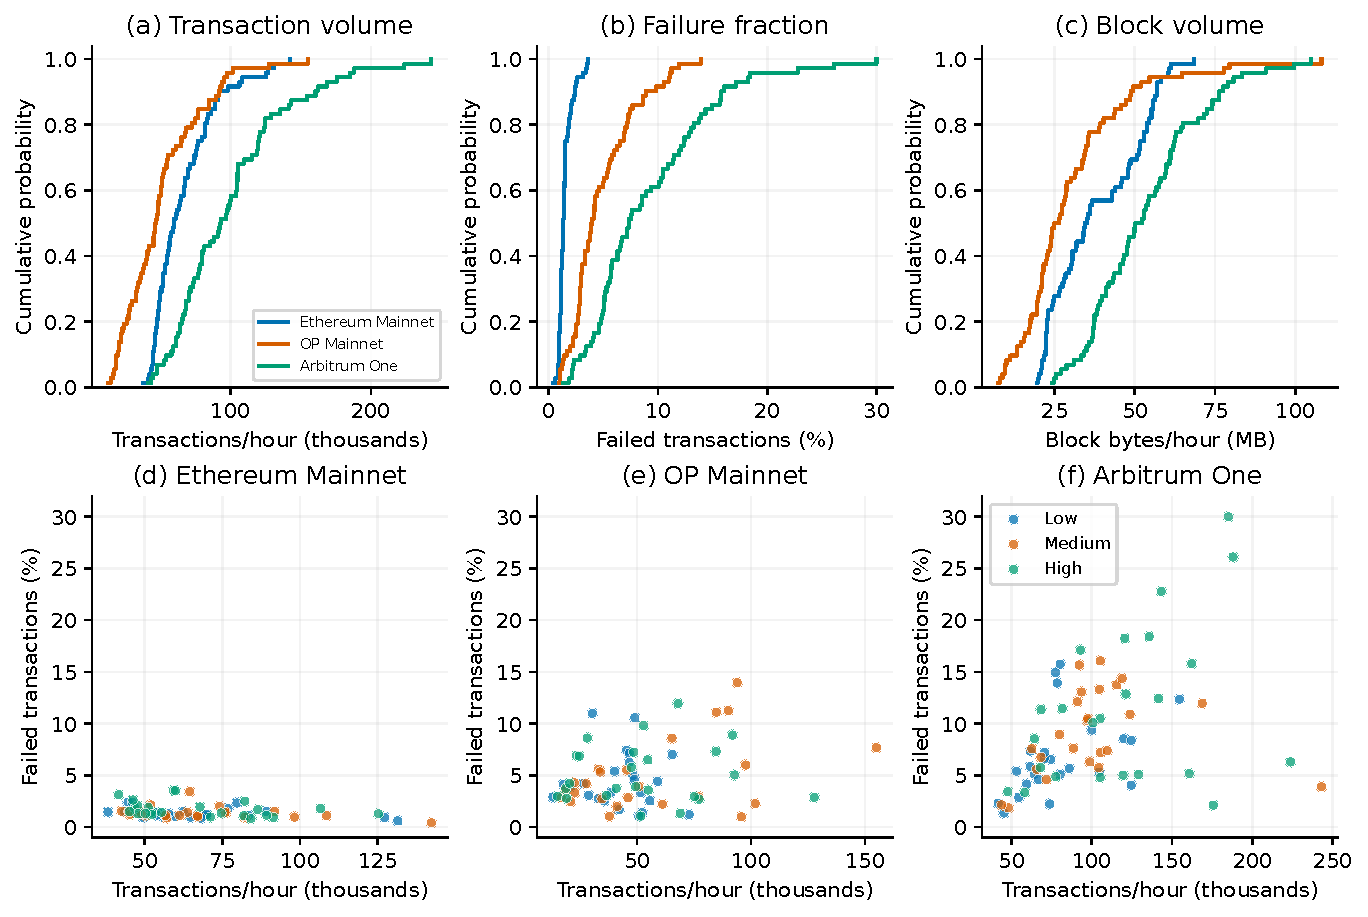
\includegraphics[width=\textwidth]{figures/workload_combined.pdf}
\caption{Workload distributions and within network load profiles across 72 probability sampled hours per network. Top row: empirical cumulative distributions of (a) transaction counts, (b) failed transaction fractions, and (c) summed block bytes, with network colors identified in panel (a). Bottom row: transaction volume versus failure fraction for (d) Ethereum Mainnet, (e) OP Mainnet, and (f) Arbitrum One. Bottom row colors indicate within phase gas rank groups, as shown in panel (f), according to gas rank. Each group contains 24 hours per network. MB denotes one million bytes.}\label{fig:workload_combined}
\end{figure}
\FloatBarrier
Figure~\ref{fig:transaction_mix} places Ethereum (E), OP Mainnet (O), and Arbitrum One (A) side by side in each phase. Pooled type 2 shares are 84.5\%, 83.9\%, and 59.2\%, respectively, weighting transactions equally. Variation in the remaining types, including the source defined other category, adds workload context. Transaction types classify envelopes, with state access and hardware traffic requiring separate measurement.

\begin{figure}[H]
\centering
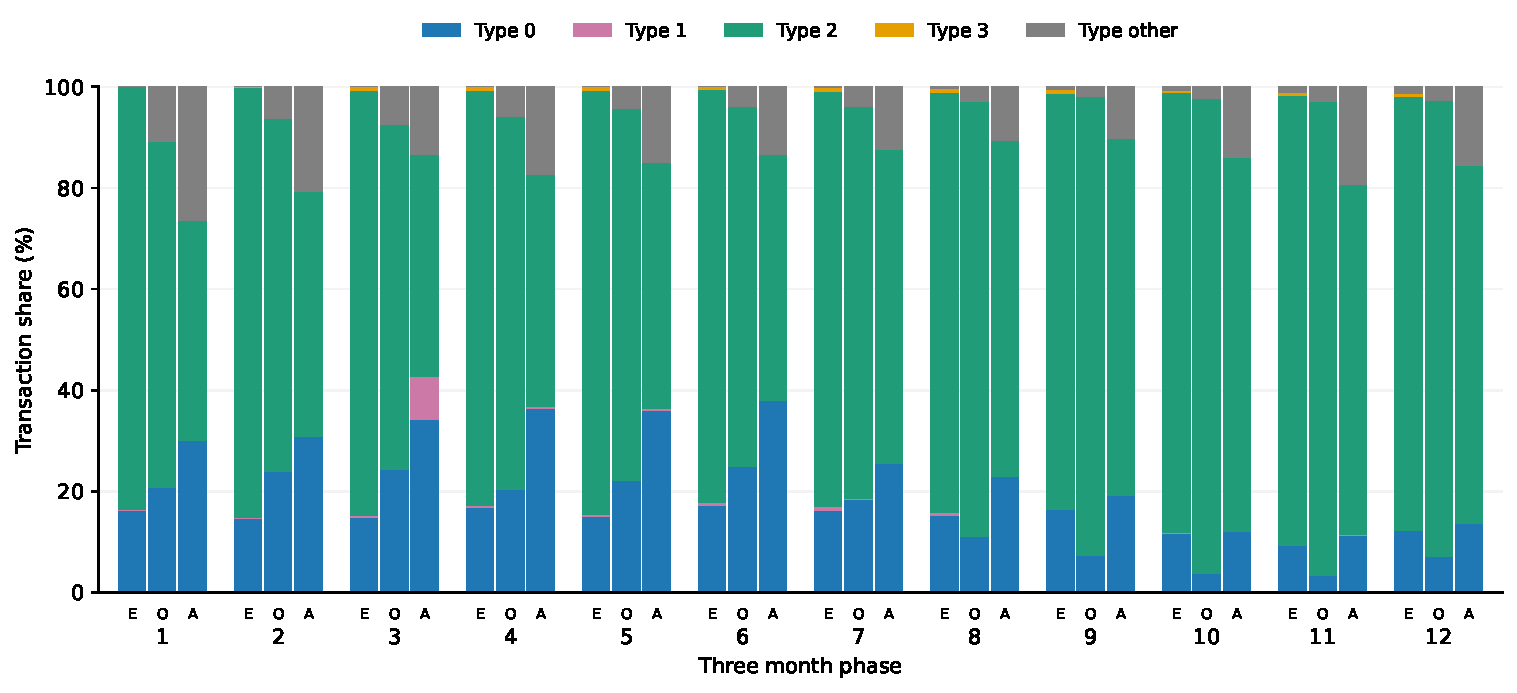
\includegraphics[width=\textwidth]{figures/transaction_mix.pdf}
\caption{Transaction type composition on one common coordinate system. Each phase shows Ethereum Mainnet (E), OP Mainnet (O), and Arbitrum One (A), from left to right. Each bar totals 100\%. Shares use summed transaction counts across the six sampled hours per phase and network. Other types retain the source dataset classification, including chain specific transaction types.}\label{fig:transaction_mix}
\end{figure}
\FloatBarrier
Figure~\ref{fig:correlations} summarizes joint variation in workload indicators across the same 72 hours per network. Associations among volume, failures, and data size can guide replay selection. Pooled correlations also reflect phase changes, so execution evidence is needed to attribute communication overhead.

\begin{figure}[H]
\centering
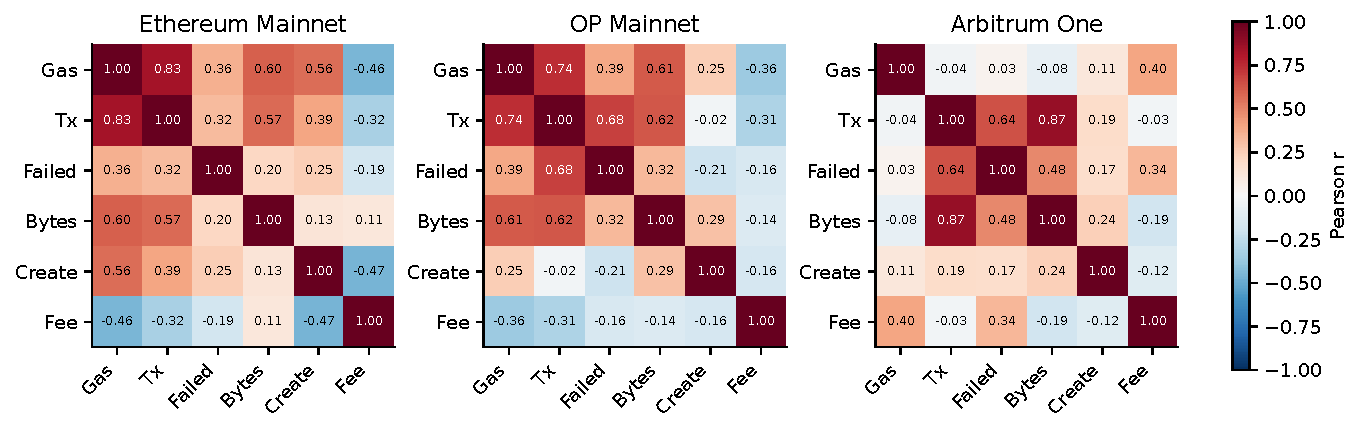
\includegraphics[width=\textwidth]{figures/correlations.pdf}
\caption{Within network Pearson correlations across 72 hourly observations. Gas, Tx, Failed, Bytes, and Create are hourly sums. Fee is the arithmetic mean of block base fees in the hour. Correlations are unweighted and pooled across phases, so temporal changes can affect their values. The correlations summarize descriptive associations.}\label{fig:correlations}
\end{figure}
\FloatBarrier
\section{Architecture and Evaluation Methodology}

We define an eight module topology, derive proxy weights from normalized block and receipt aggregates, and compare placements under a common cost objective. Training dates determine placements and held out dates evaluate them. Replay and calibrated trace mapping remain future stages. Section~5 reports the constructed matrices and layout results.

\subsection{Minimal Accelerator Model}
Table~\ref{tab:modules} defines the eight modules and their interfaces. Data widths, bandwidths, latencies, and buffering require calibration before timing evaluation. Interface calibration and RTL validation remain subsequent stages of this architecture level model.
\begin{table}[H]
\caption{Candidate modules and interface roles in the initial architecture.}\label{tab:modules}
\small\centering
\begin{tabularx}{\textwidth}{@{}lX@{}}
\toprule Module & Intended input and output role \\\midrule
Instruction dispatch & Decode instructions and issue commands to execution and state units.\\
Stack & Supply 256-bit operands and receive execution results.\\
Arithmetic unit & Consume operands and return arithmetic or logical results.\\
Keccak unit & Consume byte sequences and return hashes.\\
Memory & Serve execution memory reads, writes, and hashing inputs.\\
State controller & Translate account/storage requests into state access operations.\\
Cache & Serve cached state data and forward misses or writebacks.\\
External memory interface & Exchange memory requests and responses with off chip storage.\\
\bottomrule
\end{tabularx}
\end{table}
\FloatBarrier
For modules $b_i$ and $b_j$, static connectivity follows the Rect3D formulation~\cite{rect3d}:
\begin{equation}
A_{ij}=\sum_{e:\{b_i,b_j\}\subseteq S_e}c_e \quad(i\ne j),\qquad A_{ii}=0\label{eq:connectivity}
\end{equation}
Here $S_e$ contains the modules attached to connection $e$, and $c_e$ is its weight. We assume twelve undirected unit connections shared across all networks. Thus $A$ is a symmetric $8\times8$ binary matrix with a zero diagonal. It specifies the assumed architecture shared by the workloads.

\subsubsection{Workload informed proxy weights}
For each sampled chain hour $w$, transaction count, contract creation count, and summed block bytes are normalized within the network to obtain $X_{\mathrm{tx}}^{(w)}$, $X_{\mathrm{create}}^{(w)}$, and $X_{\mathrm{bytes}}^{(w)}$. The primary mapping is
\begin{equation}
W_{ij}^{(w)}=A_{ij}\left(1+\alpha_{ij}X_{\mathrm{tx}}^{(w)}+\beta_{ij}X_{\mathrm{create}}^{(w)}+\gamma_{ij}X_{\mathrm{bytes}}^{(w)}\right)\label{eq:proxy}
\end{equation}
The coefficients are fixed before optimization. Transaction counts proxy general execution activity, creations proxy potential deployment related state and hashing work, and bytes proxy data volume. Operation and transfer counts require execution evidence. Gas used serves only for load grouping.

Coefficient triplets $(\alpha,\beta,\gamma)$ apply symmetrically. Dispatch with stack, dispatch with arithmetic, and stack with arithmetic use $(1,0,0)$. Dispatch with Keccak uses $(0,1,0)$. Dispatch with memory and stack with memory use $(1,0,1)$. Dispatch or stack with the state controller, and the state controller with cache, use $(1,1,0)$. Memory with Keccak uses $(0,1,1)$. Cache or memory with the external memory interface uses $(0,0,1)$.

The mapping preserves the sparsity, symmetry, and zero diagonal of $A$. Its baseline retains each connected edge when normalized inputs are zero. The same hourly matrix is used across layouts. These dimensionless proxy weights differ from the directed traffic bytes in $T^{(w)}$.

\subsection{Replay Sample Selection}
Block identifiers, timestamps, gas use, and transaction counts guide replay selection across twelve phases and three load groups per chain. A small pilot will precede expansion. The earlier nine block manifest used whole period load ranks and requires reconciliation with the probability calendar and phase groups before formal evaluation.

\subsection{Execution Tracing and Communication Mapping}
Replay requires historical state and transactions or detailed compatible node traces. Block hashes and transaction counts must match collection records. Traces must expose operations, operands, execution depth, memory lengths, and state accesses, accounting for precompiles and network specific rules.

Trace mapping will record each event's source, destination, bytes, and time or cycle. For workload $w$, directed traffic is
\begin{equation}
T_{ij}^{(w)}=\sum_{k\in\mathcal{E}_{ij}^{(w)}}q_k\label{eq:traffic}
\end{equation}
Here $\mathcal{E}_{ij}^{(w)}$ contains events from $i$ to $j$, and $q_k$ is the transferred byte count. The matrix may be asymmetric and must sum to total event bytes. Cache behavior, state representation, and routing govern the events associated with operations such as \texttt{SLOAD}. Reverted execution also incurs work and communication. This stage awaits implementation, with Eq.~\eqref{eq:stratified} serving the separate statistical analysis.

\subsection{Controlled Layout and Performance Comparison}
We compare baseline planar, optimized planar, and optimized two layer assignments using identical modules and fixed slot geometries. Weights are $W=A$ for the static pilot and Eq.~\eqref{eq:proxy} for the proxy experiment. Within each phase, seed 20231116 selects two weekdays and one weekend for testing, leaving three dates for training. The partition uses probability dates, giving 36 training and 36 test hours per network.

Each feature is normalized by subtracting its training 5th percentile, dividing by the difference between its training 95th and 5th percentiles, and clipping to $[0,1]$. Equal percentiles yield 0.5. Test hours use the frozen parameters. All 216 source files pass checks for chain identity, timestamp bounds, duplicates, consecutive heights, and parent hash continuity. Independent verification of hour boundary completeness remains pending.

For placement $P$ and vertical to planar unit cost ratio $r$, communication cost is
\begin{equation}
C(P,r)=\sum_{i\ne j}W_{ij}\left[d_{xy}^{P}(i,j)+r\,d_z^{P}(i,j)\right]\label{eq:cost}
\end{equation}
Here $d_{xy}^{P}(i,j)=|x_i-x_j|+|y_i-y_j|$ is Manhattan distance in normalized slot pitches, and $d_z^{P}(i,j)=|z_i-z_j|$ is separation in layer steps. Parameter $r$ expresses their assumed unit cost conversion. Static and proxy weights yield dimensionless scores. Future weights $W=T^{(w)}$ would yield byte weighted distances. Weights remain fixed across compared placements. Ordered pairs are summed once, counting symmetric edges twice while preserving optima and relative reductions. Endpoint traffic and routed per hop traffic require distinct accounting.

The placement objective is
\begin{equation}
P^*=\underset{P\in\mathcal{P}}{\arg\min}\ C(P,r)\label{eq:optimal}
\end{equation}
The set $\mathcal{P}$ contains one to one module assignments to either a $4\times2$ planar grid or a $2\times2\times2$ grid, with equal slot counts and assumed equal module areas. Exhaustive search evaluates $8!=40{,}320$ permutations per grid, establishing an optimum only within these constraints. Sweeping $r$ compares optimized layouts, with baseline planar placement as a reference.

Timing evaluation requires compute latency, dependencies, contention, and queueing. CPU comparisons require matched operations and correctness criteria. Performance, energy, and area claims await calibrated implementation models, RTL simulation, and physical design evaluation.

\section{Experimental Results}

We report matrix construction and layout costs under static weights $W=A$ and the proxy mapping in Eq.~\eqref{eq:proxy}, using the same geometry and objective.

\subsection{Connectivity Matrix Construction}

Figure~\ref{fig:weighted_matrices} shows $A$ and proxy matrices for December 3, 2023, selected as the earliest held out date. The mapping yields 72 distinct weight vectors for Ethereum, 72 for OP Mainnet, and 70 for Arbitrum One. Coincident clipped inputs explain the repeated Arbitrum vectors. Normalization expresses activity relative to each network's training distribution.

The 216 hourly $8\times8$ matrices each retain 12 undirected connections, 24 symmetric nonzero entries, and a zero diagonal. Connected weights range from 1 to 3. Each network's mean of 36 training matrices determines its layout, which is scored on the other 36 hourly matrices. The examples, complete hourly matrices, and training means are retained in the experiment artifacts.

\begin{figure}[H]

\centering
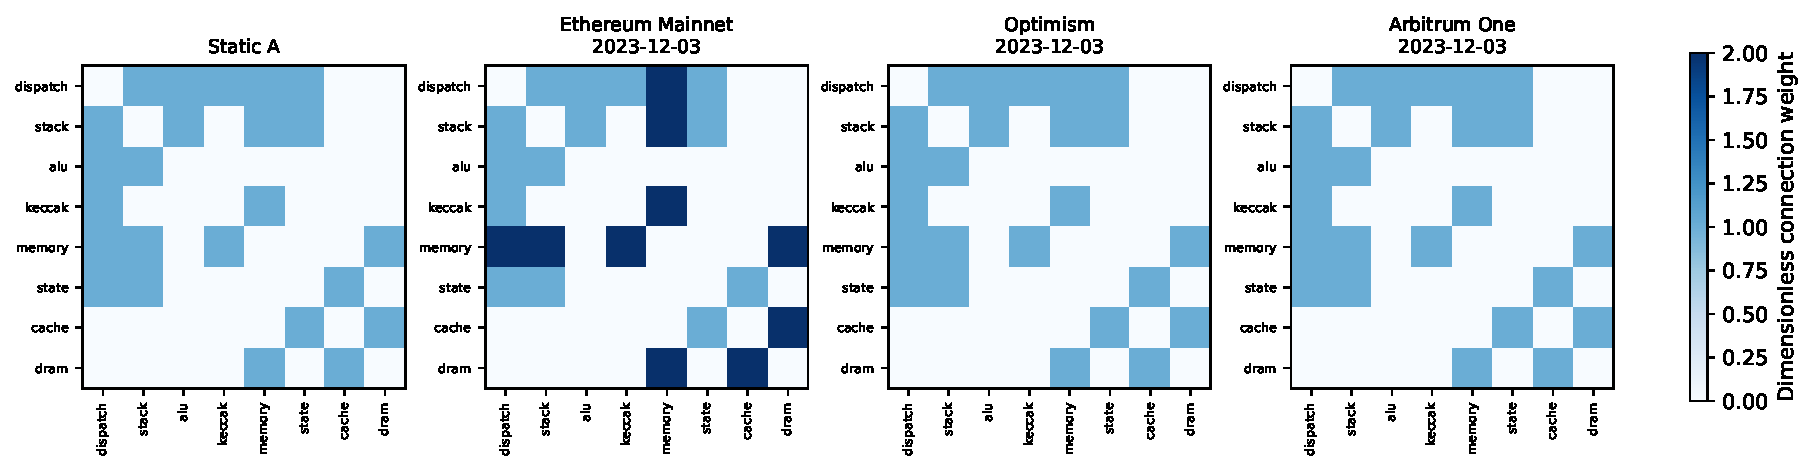
\includegraphics[width=\linewidth]{figures/weighted_matrices.pdf}
\caption{Static connectivity and example workload informed matrices. The three proxy matrices use the same held out date and the primary mapping in Eq.~\eqref{eq:proxy}. A common color scale displays dimensionless proxy weights. Module ordering is identical in all four panels.}\label{fig:weighted_matrices}

\end{figure}
\FloatBarrier
\subsection{Static Layout Evaluation}
The static experiment enumerates 40,320 assignments per grid at 161 values of $r$ from 0 to 4 in steps of 0.025. The zero endpoint is an idealized limit. Panel (a) of Fig.~\ref{fig:weighted_layout_cost} compares optimal costs and the P10 to P90 range across all labeled assignments, including geometric equivalents.

Panel (b) gives $100[32-C(P^*,r)]/32$, relative to the planar optimum of 32. Writing cost as $H_P+rV_P$, the crossing $\max_P(32-H_P)/V_P$ equals 1.25, with $V_P>0$ for every two layer assignment. Two layer cost is lower below this model specific threshold, equal at it, and higher above it.

Panel (c) separates horizontal and vertical costs, totaling 21, 30, 38, and 54 at $r=0.25$, 1, 2, and 4. Ties use the first enumerated minimizer, so component splits can vary. Panel (d) gives cost distributions across assignments. These results evaluate the weighted distance objective in Eqs.~\eqref{eq:cost} and~\eqref{eq:optimal}.

\FloatBarrier
\subsection{Workload Informed Layout Evaluation}

The workload experiment denotes $r$ by $\lambda$ and tests $\lambda\in\{0.25,1,2,4\}$. Each network's mean training matrix determines the optimum among 40,320 assignments per grid. Linearity makes this equivalent to minimizing mean training cost. Placements are then frozen for 36 test hours, retaining both directions of each symmetric edge.

Table~\ref{tab:weighted_results} reports $100(\overline{C}_{\mathrm{3D}}/\overline{C}_{\mathrm{2D,opt}}-1)$, using unweighted test mean costs. Negative values favor two layers. Optimized planar means are 51.012, 50.524, and 49.055 for Ethereum, OP Mainnet, and Arbitrum One. At $\lambda=1$, two layer means are 48.160, 48.091, and 46.481. Scores support within network layout comparisons.

\begin{table}[H]

\caption{Held out mean cost change of two layer placement relative to optimized planar placement under the primary proxy mapping. Negative values favor the two layer model.}\label{tab:weighted_results}
\centering\small
\begin{tabular*}{\linewidth}{@{\extracolsep{\fill}}lrrrr@{}}
\toprule Network & $\lambda=0.25$ & $\lambda=1$ & $\lambda=2$ & $\lambda=4$ \\\midrule
Ethereum & $-33.87\%$ & $-5.59\%$ & $+21.09\%$ & $+74.46\%$ \\
OP Mainnet & $-33.47\%$ & $-4.82\%$ & $+21.80\%$ & $+75.04\%$ \\
Arbitrum One & $-33.63\%$ & $-5.25\%$ & $+21.26\%$ & $+74.28\%$ \\
\bottomrule
\end{tabular*}

\end{table}
\FloatBarrier

A uniform scaling control multiplies every connected edge by one plus the mean of the hour's three normalized inputs. It preserves static relative changes of $-34.375\%$, $-6.25\%$, $+18.75\%$, and $+68.75\%$ at the four ratios. Differences under the functional mapping therefore reflect unequal edge reweighting.

Sensitivity analysis scales all three coefficients by $s\in\{0,0.5,1,2\}$, where zero recovers $A$ and one gives the primary mapping. Each setting is optimized on training hours and evaluated on the same test dates. Across networks and positive scales, two layer costs remain lower at $\lambda=0.25$ and 1 and higher at 2 and 4. Reductions at 1 range from 4.15\% to 5.84\%, and increases at 4 from 72.10\% to 77.95\%. These checks establish behavior at the tested settings.

\FloatBarrier

The selected planar assignment remains the static optimum across networks and scales, while weights and costs vary. Independent verification reproduces 4,320 hourly scenario costs and checks shared partitions, training normalization, matrix constraints, and test isolation. Static results are reproduced unchanged.

The results evaluate layout sensitivity under the assumed architecture and proxy mapping. Calibrated trace traffic remains necessary to relate these costs to physical communication and EVM performance.

The lower panels of Fig.~\ref{fig:weighted_layout_cost} extend the proxy evaluation to 161 ratios from 0 to 4 in steps of 0.025, using training search and test scoring. The four original ratios reproduce Table~\ref{tab:weighted_results}. Panels (e) to (h) show layout costs, planar relative reductions, horizontal and vertical contributions, and hourly cost ratios at $\lambda=1$. The zero endpoint remains idealized, and the weighted results are evaluated independently of the static crossing.

\begin{figure}[H]

\centering
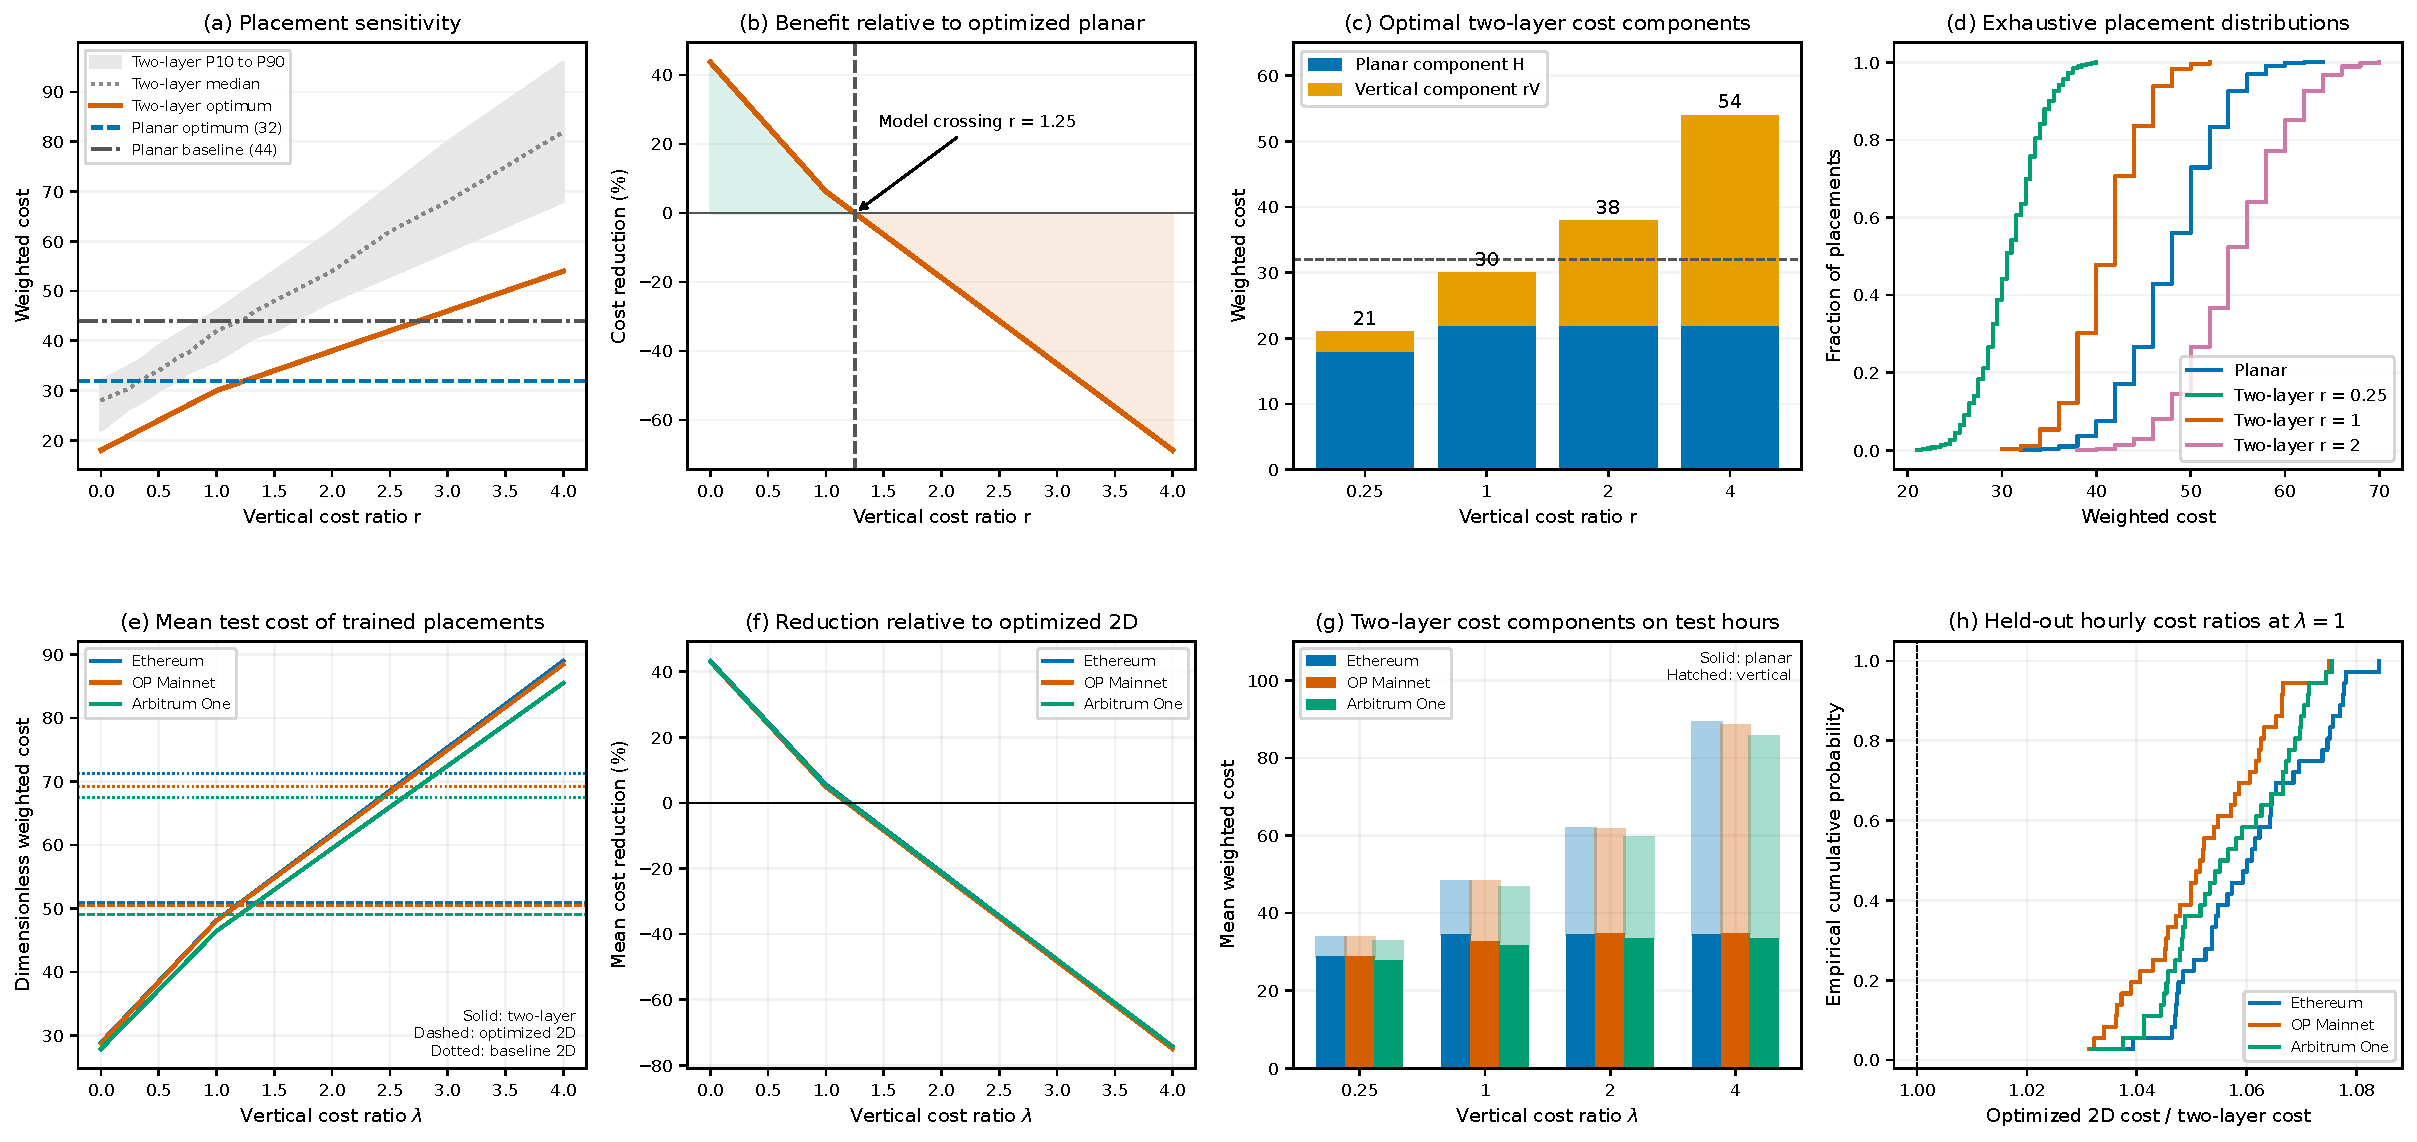
\includegraphics[width=\linewidth]{figures/layout_eight_panels.pdf}
\caption{Static and workload informed layout evaluation. Top row (a) to (d) uses unit adjacency weights: (a) placement sensitivity, (b) benefit relative to optimized planar placement, (c) horizontal and vertical costs, and (d) cost distributions across assignments. Bottom row (e) to (h) uses workload informed weights: (e) mean test costs, (f) reduction relative to optimized planar placement, (g) cost components, and (h) hourly cost ratio distributions at $\lambda=1$. Lower panels use 36 held out hours per network. Ratios express modeled communication costs.}\label{fig:weighted_layout_cost}

\end{figure}
\FloatBarrier

At $\lambda=1$, baseline planar, optimized planar, and two layer mean costs are 71.209, 51.012, and 48.160 for Ethereum, 69.165, 50.524, and 48.091 for OP Mainnet, and 67.495, 49.055, and 46.481 for Arbitrum One. Planar optimization reduces baseline costs by 26.95\% to 28.36\%. Two layers provide a further 4.82\% to 5.59\%, giving total reductions of 30.47\% to 32.37\%.

Optimized planar to two layer mean cost ratios are 1.512, 1.503, and 1.507 at $\lambda=0.25$, and 1.059, 1.051, and 1.055 at $\lambda=1$, respectively. These describe modeled communication costs. Higher costs at $\lambda=2$ and 4 make the benefit conditional on sufficiently inexpensive vertical communication. Execution speed requires separate validation.

\FloatBarrier

\section{Conclusion}
This study characterizes block production, transactions, and failures across Ethereum Mainnet, OP Mainnet, and Arbitrum One through three years of stratified sampling. An abstract eight module architecture uses transaction counts, contract creations, and block bytes as connectivity proxies. At a vertical cost ratio of one, optimized three dimensional placement reduces modeled communication costs by 5.59\%, 4.82\%, and 5.25\%, respectively, relative to optimized planar layouts.

The benefits depend on vertical costs and workload weighting assumptions. The aggregate indicators support architectural exploration, with actual hardware performance requiring validation. Future work will use EVM traces, RTL simulation, and physical design evaluation to assess communication, latency, energy, and scalability.

\begin{thebibliography}{99}
\bibitem{eip145} Beregszaszi, A., Bylica, P.: EIP-145: Bitwise shifting instructions in EVM (2017). \url{https://eips.ethereum.org/EIPS/eip-145}

\bibitem{eip1052} Johnson, N., Bylica, P.: EIP-1052: EXTCODEHASH opcode (2018). \url{https://eips.ethereum.org/EIPS/eip-1052}

\bibitem{constantinople} Ethereum Foundation: Constantinople execution specification. \url{https://steel.ethereum.foundation/docs/execution-specs/specs/reference/src/ethereum/forks/constantinople/index.html}

\bibitem{rollups} Ethereum Foundation: Optimistic rollups. \url{https://ethereum.org/en/developers/docs/scaling/optimistic-rollups/}

\bibitem{zkrollups} Ethereum Foundation: Zero knowledge rollups. \url{https://ethereum.org/en/developers/docs/scaling/zk-rollups/}

\bibitem{evmx} Lemayian, J.P., Gagnon, G., Zhang, K., Giard, P.: EVMx: An FPGA Based Accelerator for Smart Contract Processing. IEEE Transactions on Very Large Scale Integration (VLSI) Systems \textbf{34}(2), 554 to 567 (2026). \doi{10.1109/TVLSI.2025.3628118}

\bibitem{xu2013} Xu, T.C., Schley, G., Liljeberg, P., Radetzki, M., Plosila, J., Tenhunen, H.: Optimal Placement of Vertical Connections in 3D Network on Chip. Journal of Systems Architecture \textbf{59}(7), 441 to 454 (2013). \doi{10.1016/j.sysarc.2013.05.002}

\bibitem{hsu2013} Hsu, M.K., Balabanov, V., Chang, Y.W.: TSV Aware Analytical Placement for 3-D IC Designs Based on a Novel Weighted Average Wirelength Model. IEEE Transactions on Computer Aided Design of Integrated Circuits and Systems \textbf{32}(4), 497 to 509 (2013). \doi{10.1109/TCAD.2012.2226584}

\bibitem{opinterval} Optimism: OP Stack specification, Glossary. \url{https://specs.optimism.io/glossary.html}

\bibitem{rect3d} Ren, S., et al.: Rect3D: A Unified Analytical Framework for 3D IC Rectilinear Floorplanning. arXiv:2609.18946 (2026). \url{https://arxiv.org/abs/2609.18946}
\end{thebibliography}
\end{document}
